\subsection{Die Bandstruktur}
\label{sec:bandstruktur}

Um Halbleiter zu verstehen, muss zunächst einmal der Ursprung der Bandstruktur 
erklärt werden. Ein Elektron, welches sich in einem gebunden Zustand an ein 
Atom befindet, befindet sich auf einem Energieniveau. Am energetisch günstigsten 
ist es für das Elektron im Ruhezustand, das niedrigste Niveau zu besetzen. Um auf 
ein höheres Niveau zu kommen, muss Energie zugeführt werden. Die einzelnen Bahnen 
eines Atoms representieren dabei jeweils ein Energieniveau. \par 

Wird nun ein Material betrachtet, in dem mehrere Atome in unmittelbarer 
Nähe zueinander plaziert sind, beeinflussen sich die Potentialtöpfe bzw. die 
Energieniveaus untereinader und eine Aufspaltung tritt auf. In Abbildung 
\ref{fig:bandstruktur} ist dies für zwei Atome schematisch dargestellt.


\begin{figure}
  \centering
  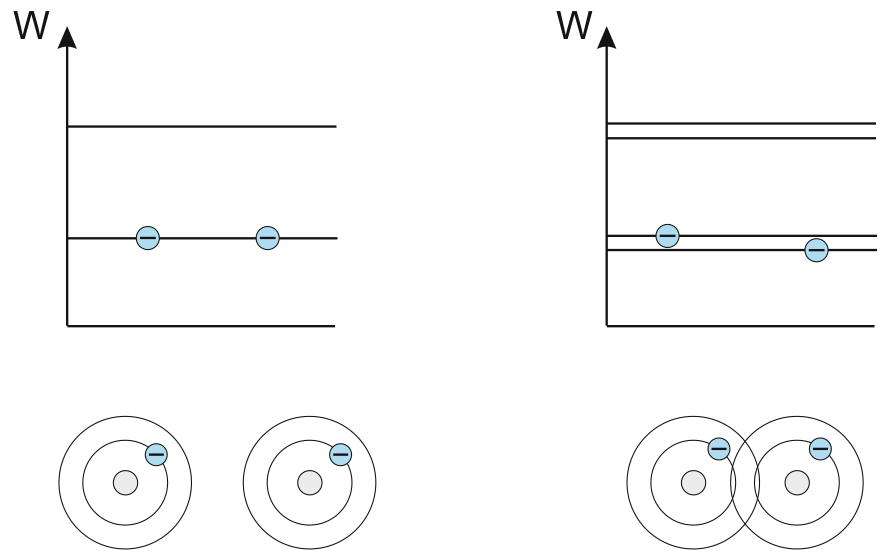
\includegraphics[width=0.7\textwidth]{content/graphics/bandstruktur.png}
  \caption{Erklärung zur Entstehung von Energiebändern. Bei der Linken Darstellung 
  muss angemerkt werden, dass nach dem Pauli Prinzip verboten ist, dass sich 
  zwei Teilchen mit exakt gleichen Quantenzahlen auf dem gleichen Energieniveau 
  befinden. Dies soll der Potentialtopf auch nicht verdeutlichen, sondern, dass 
  jedes Atom für sich bei ausreichend Abstand einen unbeinflussten 
  Potentialtopf besitzt \cite{BANDSTRUKTUR}.}
  \label{fig:bandstruktur}
\end{figure}

In einem Material beeinflussen sich allerdings nicht nur zwei Atome, sondern 
mehrere, wodurch eine Vielzahl von Aufspaltungen stattfindet. Diese 
Aufspaltungen werden dann nicht mehr als diskrete Energieniveaus beschrieben, 
sondern können als Energiebänder zusammengefasst werden. Das letzte voll 
gefüllte Band wird das Valenzband genannt und das obere, nicht vollständig 
besetzte Band, das Leitungsband. Die Bandlücke dazwischen verdeutlicht einen 
verbotenen Bereich, da dort keine Energieniveaus oder Zustände vorhanden sind, 
die besetzt werden können.